\section{Markov-Decision Process}

\orange{MDP formally describes environment, where environment is fully observable}, i.e. current (agent's) state completely characterizes that process, how the process unfolds.


Almost all RL problems can be formalized as MDPs:
\begin{itemize}
	\item Optimal control primarily deals with continuous MDPs (with continuous actions).
	\item POMDP can be converted to MDP	.
	\item \textit{Bandits} are MDPs with one state.
\end{itemize}


\boxedtext{
$$
	 \underset{\text{State chain}}{\text{Markov process}}
	 \to 
	 \underset{\text{+reward function}}{\text{Markov Reward Process}} 
	 \to
	 \underset{\text{+actions}}{\text{Markov Decision Process}}
$$
}

\subsection{Markov Process (MP)}

\red{Markov Property}: future is independent of the past given present.

\begin{align}
	\Prob[S_{t+1} | S_t] = 	\Prob[S_{t+1} | S_t, S_{t-1}, ..., S_{0}]
\end{align}

It means that we can define a \red{state-transition probability matrix}
\begin{align}
	\TransitionProb_{ss'} = \Prob[S_{t+1} = s' | S_t = s]
\end{align}

\boxedtext{
\red{Markov Process (Markov Chain)} is a memory-less process defined as a tuple $\MP=(\mathcal{S}, \mathcal{P})$:
\begin{itemize}
	\item $\States$ is a (finite) set of states;
	\item $\TransitionProb$ is state transition probability matrix: $\TransitionProb_{ss'} = \Prob[S_{t+1} = s' | S_t = s]$
\end{itemize}

This fully defines dynamics of the system.
}


\begin{notebox}
What to do if probability matrix change in time? Non-stationary Markov process (or non-stationary MDP in general).


\begin{enumerate}
	\item  You can use the same algorithms we use in the stationary case but incrementally adjust your solution to track the best solution you've found so far.
	\item or you can reduce non-stationary dynamics to a more complex Markov process \gray{(see 12:00 of the video with Facebook example, where probability of staying on Facebook reduces with time or number of visits)}
\end{enumerate}
\end{notebox}


\subsection{Markov Reward Process}
\label{sec:MRP}
\red{Markov Reward Process (MRP)} is a Markov chain with values defined as a tuple $\MRP = (\States, \TransitionProb, \red{\Reward, \gamma})$:
\begin{itemize}
	\item $\Reward$ is a \red{reward function}: $\Reward_s = \E[R_{t+1} | S_t = s]$
	\begin{itemize}
		\item how much (expected) reward do I get from simply being in that state;
	\end{itemize}
	\item $\gamma$ is a \red{discount factor} $\gamma \in [0, 1]$
\end{itemize}
\emph{Reward function} allows us to value how much reward I accumulate \textit{across a particular sequence} sampled from this Markov process.


The \red{return $G_t$} is the total discounted reward from time-step $t$ (\underline{across entire chain}).
\begin{align}
	G_t = R_{t+1}+ \gamma R_{t+2} + \gamma^2 R_{t+3} ... = \sum_{k=0}^{\infty} \gamma^k R_{t+k+1}
\end{align}

\begin{notebox}
Why use discount factor $\gamma$?
\begin{itemize}
	\item admit the fact that our model is imperfect, hence future is more uncertain than present;
	\begin{itemize}
		\item we build $\MRP$ to represent environment, but it is imperfect model of the environment;
		\item if we build a long plan that says I have to wait for many steps before collecting a large reward, I have to really trust my model and really believe that things will turn out as I plan to wait for so long...
	\end{itemize} 
	\item \orange{$\gamma$ helps to define $G_t$ to converge to finite!!}
	\begin{itemize}
		\item avoids infinite returns $G$ in cyclic $\MRP$;
		\item makes sure there is no infinite evaluation of a state.
	\end{itemize}
	\item \textit{Myopic} ($\gamma=0$) vs \textit{far-sighted} ($\gamma=1$)
	\begin{itemize}
		\item we introduce a judgement here - we prefer a short-term reward to delayed reward and amount is given by $\gamma$;
		\item the way to interpret $\gamma$ is that we effectively look $\frac{1}{1-\gamma}$ steps into the future.
	\end{itemize}
	\item if the reward is financial, then money now worth more than money later (interest);
	\item \orange{it is sometimes possible to use \textit{undiscounted} ($\gamma=1$) MRPs, e.g. if we know that all sequences terminate.}
	\begin{itemize}
		\item approach: average reward formulation
	\end{itemize}
\end{itemize}
\end{notebox}

\subsubsection{Value Function and Bellman Equation for MRPs}

\red{Value Function} $v(s)$ of $\MRP$ gives long-term value of a state $s$
\begin{align}
	v(s) = \E[G_t | S_t = s]
\end{align}
\begin{itemize}
	\item If I drop you into the state $s$ of this MRP, what is the expected total reward I am going to collect?
	\item We use expectation, because environment is stochastic.
\end{itemize}

\boxedtext{
The value function can be decomposed into two parts:
\begin{itemize}
	\item expected immediate reward $R_{t+1}$;
	\item expected discounted value of successor state $\gamma v(S_{t+1})$.
\end{itemize}

\begin{align*}
	v(s) &= \E[G_t | S_t = s] = \E[R_{t+1} + \underbrace{\gamma R_{t+2} + \gamma^2 R_{t+3} + ...}_{\gamma G_{t+1}} | S_t = s ] \\
	     &= \E[R_{t+1} | S_t = s] + \gamma \E[\underbrace{\E[G_{t+1}|S_{t+1} = s', \cancel{S_t = s}]}_{v(s')} | S_t = s] \\
	     &= \E[R_{t+1} | S_t = s] + \gamma \E[v(S_{t+1}) | S_t = s]
\end{align*}
}

\begin{notebox}
	Why immediate reward when we exit state $S_t$ is $R_{t+1}$? That's just a convention about when tick-counter gets updated. In this convention tick is updated at when environment takes control and emits reward and observation.
\end{notebox}

\red{Bellman equation} is a tautological definition of value function and can be though as a \red{one step look-ahead search} (backup diagram).



\begin{minipage}{0.5\textwidth}

\begin{align*}
	v(s) & = \E[R_{t+1} + \gamma v(S_{t+1})| S_t = s] \\
	     & \Updownarrow \\
	v(s) & = \mathcal{R}_s + \gamma \sum_{s' \in \mathcal{S}} \mathcal{P}_{s s'} v(s') \\
\end{align*}
\end{minipage}
\begin{minipage}{0.5\textwidth}
	    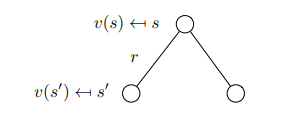
\includegraphics[width=0.8\textwidth]{img/mrp_bellman_diagram}
\end{minipage}


\boxedtext{
In matrix form

\begin{align}
	v &= \mathcal{R} + \gamma \mathcal{P} v \\
	\statevector &= \rewardvector + \gamma \probmatrix \statevector \nonumber
\end{align}

It is a linear equation and can be solved directly
\begin{align}
	v = (I - \gamma \mathcal{P})^{-1} \mathcal{R}
\end{align}

\begin{itemize}
	\item Complexity is $\bigO(n^3)$, so can only be solved for small problems.
	\item For larger problems there are other methods
	\begin{itemize}
		\item Dynamic programming;
		\item Monte-Carlo evaluation;
		\item Temporal-Difference learning.
	\end{itemize}
\end{itemize}
}

\subsection{Markov Decision Process (MDP)}
\orange{This is the thing we are actually solving in RL}

MDP = MRP + actions

\boxedtext{
\red{Markov Decision Process (MDP)} is a tuple $\red{\MDP}=(\States, \red{\Actions}, \TransitionProb, \Reward, \gamma)$
\begin{itemize}
	\item $\States$ is a finite set of states;
	\item \red{$\Actions$ is a finite set of actions;}
	\item $\TransitionProb$ is a state transition prob matrix (\red{may depend on action})  $$\TransitionProb_{ss'}^{\red{a}} = \Prob[S_{t+1} = s' | S_t = s, A_t = \red{a}]$$
	\item $\Reward$ is a reward function (\red{may depend on action}): $$R_s^{\red{a}} = \E[R_{t+1} | S_t = s, A_t = \red{a}]$$
	\item $\gamma$ is a discount factor.
\end{itemize}

\orange{There is much more control now for agent to control the path over the states (\red{agency})}

}

\boxedtext{
A (stochastic) \red{policy} is a distribution over actions given state
\begin{align}
	\pi(a|s) = \Prob[A_t=a | S_t = s]
\end{align}
\begin{itemize}
	\item \orange{This is something that agent controls!}
	\item A policy fully defines \textit{behavior} of an agent;
	\item it is convenient to make it stochastic to later introduce \textit{exploration}.
	\item \red{Markov property}: in MDP, policy depends only on the current state, not on the history\footnote{Reminder: Markov assumption says that future is fully characterized by current state}. as a result we consider \textit{stationary policies}: $\forall t: A_t \sim \pi(\cdot|s_t)$
	\item \red{to follow a policy $\pi$} means we sample actions from $A_t \sim \pi(a|S_t)$
\end{itemize}
}
\linebreak

\boxedtext{
	\orange{\textbf{Important reductions}}
	
	If I have an $\MDP=(\States, \Actions, \TransitionProb, \Reward, \gamma)$ and a (fixed) policy $\pi(a|s)$, then
	
	\begin{itemize}
		\item $MDP \to MP^{\pi}$: the state sequence $S_1, S_2, ...$ defines a $\MP^{\pi}=(\States, \red{\TransitionProb^{\pi}})$
		\item $MDP \to MRP^{\pi}$: the state-reward sequence $S_1, R_2, S_2, R_3, ...$ defines a $\MRP^{\pi}=(\States, \red{\TransitionProb^{\pi}}, \red{\Reward^{\pi}}, \gamma)$
	\end{itemize}
where we \orange{just average over the policy}:
\begin{align}
	\red{\TransitionProb^{\pi}_{ss'}} &= \sum_{a \in\Actions} \pi(a|s) \TransitionProb_{ss'}^a \gray{ = \sum_{a \in\Actions} \Prob[A_t=a|S_t=s] \Prob[S_{t+1} = s' | S_t=s, A_t = a] }\\
	\red{\Reward^{\pi}_{s}} &= \sum_{a \in\Actions} \pi(a|s) \Reward_s^{a}  \gray{(see \ref{sec:MRP})}
\end{align}
}

\subsubsection{State-value and Action-value functions for MDP}
Our previous definition of value function worked for a $\MRP$, where we just flew through the states but did not have any control (agency). There is no single expectation, expectation depends on behavior we choose. We need to redefine notion of value function. We can do that if we \underline{fix the policy $\pi$}.

%\boxedtext{
The \red{\textit{state}-value function $v_\pi(s)$} of an $\MDP$ is the expected return given I start at state $s$ and then follow the policy $\pi$:
\begin{align}
	v_{\red{\pi}}(s) = \E_{\red{\pi}}[G_t | S_t = s]
\end{align}
\begin{itemize}
	\item subscript \red{$\pi$} means that we follow the policy $\pi$ after we live the state $S_t$;
	\item it is same as the value function of policy-induced $\MRP^{\pi}$
	\item \orange{meaning: how good it is to be in state $s$ if we follow policy $\pi$}
\end{itemize}

The \red{\textit{action}-value function $v_\pi(s)$} of an $\MDP$ is the expected return given I start at state $s$, make action $a$ and then follow the policy $\pi$:
\begin{align}
	q_{\red{\pi}}(s, a) = \E_{\red{\pi}}[G_t | S_t = s, A_t=a]
\end{align}
\begin{itemize}
	\item subscript \red{$\pi$} means that we follow the policy $\pi$ after we live the state $S_t$;
	\item it is the quantity we are intuitively most interested in when selecting optimal action
	\item \orange{meaning: how good it is to take action $a$ from state $s$ if we follow policy $\pi$}
\end{itemize}
%}

\subsubsection{Bellman equation}
Again, same idea, the value function can be decomposed into expected immediate reward plus expected value of successor state given we follow the policy $\pi$. Same works for state- and action- value functions.

One-step lookaheads give us relation between $v$ and $q$ functions.

\boxedtext{
\begin{minipage}{0.75 \textwidth}
\begin{align*}
	v_{\pi}(s) &= \E_{\pi}[G_{t} | S_t = s] \\
			   &= \E_{A_t \sim \pi(a|s)} \Big[ \underbrace{\E_{\pi}[G_{t} | S_t = s, A_t = a]}_{q_{\pi}(s, a)}\Big] \\
			   &= \sum_{a\in \Actions} \pi(a|s) q_{\pi}(s, a)
\end{align*}
\end{minipage}
\begin{minipage}{0.22 \textwidth}
		    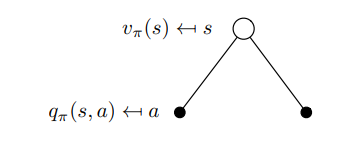
\includegraphics[width=\textwidth]{img/mdp_bellman_1}
\end{minipage}
}

\boxedtext{
\begin{minipage}{0.7 \textwidth}
	\begin{align*}
		q_{\pi}(s, a) &= \E_{\pi}[G_{t} | S_t = s, A_t = a] \\
		&= \E_{\pi}[R_{t+1} + \gamma G_{t+1} | S_t = s, A_t = a] \\
		&= \Reward_s^a + \gamma \E_{s' \sim S_{t+1}|S_t=s,A_t=a} \Big[\underbrace{\E_{\pi}[G_{t+1} | S_{t+1} = s', \cancel{S_t = s, A_t = a}]}_{v_{\pi}(s')}\Big] \\
		&= \Reward_s^a + \gamma \sum_{s'\in \States} \TransitionProb_{ss'}^a v_{\pi}(s')
	\end{align*}
\end{minipage}
\begin{minipage}{0.22 \textwidth}
	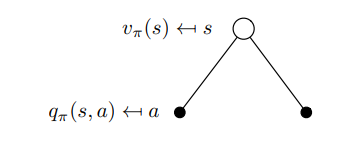
\includegraphics[width=\textwidth]{img/mdp_bellman_1}
\end{minipage}
}

Combining the two we get

\boxedtext{
	\begin{minipage}{0.75 \textwidth}
		\begin{align*}
			v_{\pi}(s) &= \underbrace{\sum_{a\in \Actions} \pi(a|s) \Reward_s^a}_{\E_{\pi}[R_{t+1} | S_t=s]} + \gamma \underbrace{\sum_{a\in \Actions} \pi(a|s) \sum_{s' \in \States} \TransitionProb_{ss'}^a v_{\pi} (s')}_{\E_{\pi}[v(S_{t+1}) | S_t = s]}
		\end{align*}
	\end{minipage}
	\begin{minipage}{0.22 \textwidth}
		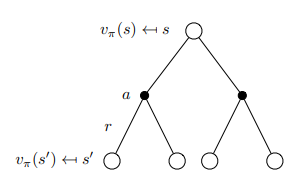
\includegraphics[width=\textwidth]{img/mdp_2step_lookahead_pi}
	\end{minipage}
}

and 

\boxedtext{
	\begin{minipage}{0.75 \textwidth}
		\begin{align*}
			q_{\pi}(s, a) &= \underbrace{\Reward_s^a}_{\E_{\pi}[R_{t+1} | S_t=s, A_t = a]} + \gamma \underbrace{\sum_{s'\in \States} \TransitionProb_{ss'}^a \sum_{a' \in \Actions} \pi(a'|s') q_{\pi} (s', a') }_{\E_{\pi}[q_{\pi}(S_{t+1}, A_{t+1})|S_t=s, A_t=a]}
		\end{align*}
	\end{minipage}
	\begin{minipage}{0.22 \textwidth}
		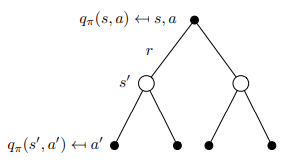
\includegraphics[width=\textwidth]{img/mdp_2step_lookahead_q}
	\end{minipage}
}

\boxedtext{
The Bellman equation can be expressed in matrix form using $\pi$-induced MRP:

\begin{align*}
	v_{\pi} = \Reward^{\pi} + \gamma \TransitionProb^{\pi} v_{\pi} \\
\end{align*}

with direct solution

\begin{align*}
	v_{\pi} = (I-\gamma \TransitionProb^{\pi})^{-1} \Reward^{\pi}
\end{align*}
}

\subsection{Optimal Value Function}

The \red{optimal state-value function $v_*(s)$} is the maximum state-value function over all policies:
\begin{align*}
	v_*(s) = \max_{\pi} v_{\pi}(s)
\end{align*}

The \red{optimal action-value function $q_*(s, a)$}  is the maximum action-value function over all policies:
\begin{align*}
	q_*(s, a) = \max_{\pi} q_{\pi}(s, a)
\end{align*}

\orange{Once we know $q_*(s, a)$, we immediately get $\pi_*$!}

\begin{notebox}
	In the transition diagram:
	\begin{itemize}
		\item $v_\pi(s)$ are assigned to nodes (states);
		\item $q_\pi(s, a)$ are assigned to edges/arcs (action from a particular state).
	\end{itemize}
\end{notebox}
